\documentclass[../Supercritical_fluid_extraction_of_essential_oil_from_chamomile.tex]{subfiles}
\graphicspath{{\subfix{../Figures/}}}
\begin{document}
	
	\label{CH: Results}
	
	The parameter estimation problem was solved multiple times for different initial guesses. Each time series was fitted to the model separately. First, the model with linear extraction kinetics was the only one fitted to the dataset. The Figure shows the parameter estimation result for dataset 1, corresponding to the following operating conditions: $40^\circ C$, 100 bar and 6.67$\times 10^{-5}$ kg/s.
	
	\begin{figure}[!h]
		\centering
		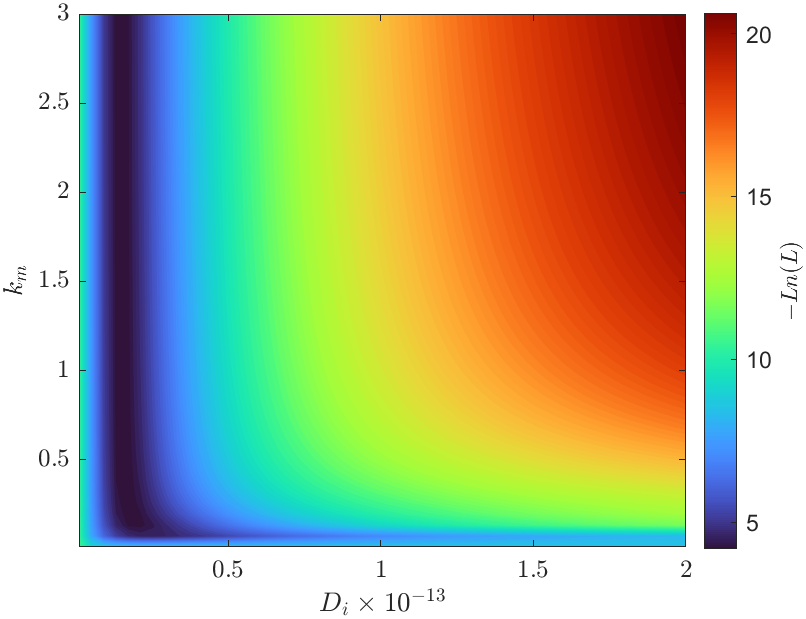
\includegraphics[trim = 0.0cm 0.0cm 0.0cm 0.0cm,clip, width=\columnwidth]{/Results_estimation/Parameter_Space_Linear_Dataset_1.png}
		\caption{Parameter space for the linear extraction kinetic model and the experiment 1}
		\label{fig: Fit_1_linear}
	\end{figure}
	
	In the case of the model with linear kinetic, two parameters are unknown, namely the partition coefficient $k_m$ and the internal diffusion coefficient $D_i$. Figure \ref{fig: Fit_1_linear} shows the cost function's parameter space and corresponding values. As the cost function is to be minimized, the lowest value of $-\ln(L)$ indicate the best fit. A black vertical stripe at $D_i \approx 0.2$ can be observed. That stripe indicates the existence of the optimal value of the $D_i$. In the direction of $k_m$, the cost function is almost flat, which suggests that any value of $k_m$ above 0.1 fits the data equally well. If $k_m$ can be an arbitrary point, then it can grow to infinity, which suggests that the solvent is far from the saturation, and the model can be simplified. The model reduction can be introduced by considering the limit of $k_m$ in the extraction kinetic term: 
	
	{\footnotesize
		\begin{equation*}
			\begin{split}
				&\lim_{k_m \rightarrow \infty} \left({\color{black}{\color{black} c_s} }(t,z)  - \cfrac{{\color{black}\rho_s}}{{\color{black}k_m}({\color{black}T}(t,z)){\color{black}\rho}({\color{black}T}(t,z),{\color{black}P}(t))}  {\color{black}c_f}(t,z) \right)  = \\
				&= \left({\color{black}{\color{black} c_s} }(t,z)  - \cfrac{{\color{black}\rho_s}}{\infty{\color{black}\rho}({\color{black}T}(t,z),{\color{black}P}(t))}  {\color{black}c_f}(t,z) \right) = \left({\color{black}{\color{black} c_s} }(t,z) - 0 \right)
			\end{split}
	\end{equation*} }
	
	The extraction model can be modified to account for the reduced kinetic term and the axial diffusion. In such a configuration, two parameters are unknown: internal diffusion coefficient $D_i$ and axial diffusion coefficient $D_e^M$. Figure \ref{fig: Fit_1_Di_Dx} shows the parameter space and corresponding values of the cost function.
	
	\begin{figure}[!h]
		\centering
		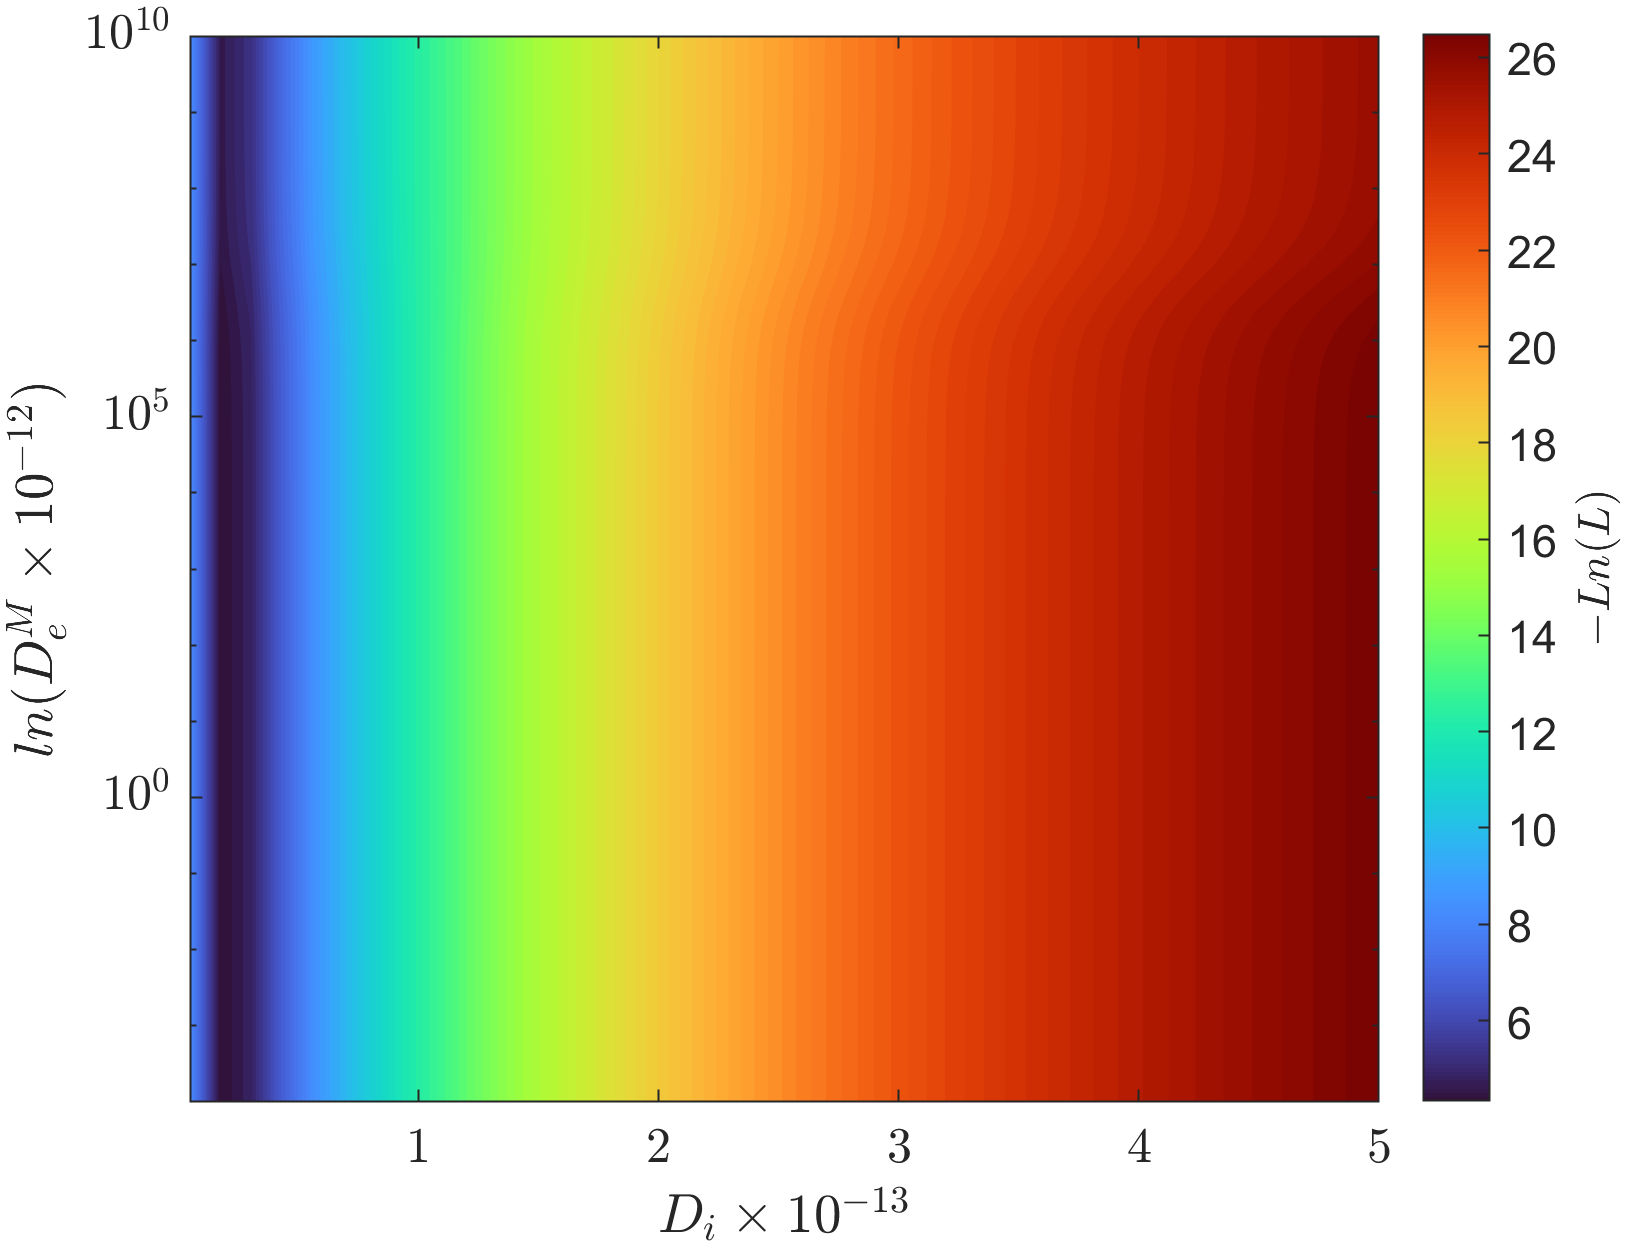
\includegraphics[trim = 0.0cm 0.0cm 0.0cm 0.0cm,clip, width=\columnwidth]{/Results_estimation/Parameter_Space_Di_Dx_Dataset_1.png}
		\caption{Parameter space for the reduced linear extraction kinetic model with and the experiment 1}
		\label{fig: Fit_1_Di_Dx}
	\end{figure}
	
	Similarly to the previous case, the optimal value of $D_i$ exists, but a unique value for the $D_e^M$ cannot be determined. A little influence of the axial diffusion coefficient can be observed in Figure \ref{fig: Fit_1_Di_Dx} in a width range of values. By selecting $D_e^M$, which has a low value, the axial diffusion term can be reduced and removed from the model without losing generality. Similar was drawn by \citet{Rahimi2011}, who worked with the same dataset and obtained Peclet numbers from 290 to 400. Such high values of the Peclet number suggest that the advection term dominates the mass transfer, and the axial diffusion is negligible.
	
	In both cases discussed above, none of the fitting results were satisfactory. Following the idea behind the Broken-and-Intact and Shrinking Core models (presented in Chapter \ref{CH: Gamma_Function}), the gamma function is introduced to account for the decaying extraction kinetic. The proposed correction factor is combined with the reduced linear model, which leads to a new two-parameter ($D_i^R$ and $\Upsilon$) model defined by Equation \ref{Model_kinetic}. Figure \ref{fig: Fit_1_Di_Dx} shows the parameter space with and the corresponding values of the cost function.
	
	\begin{figure}[!h]
		\centering
		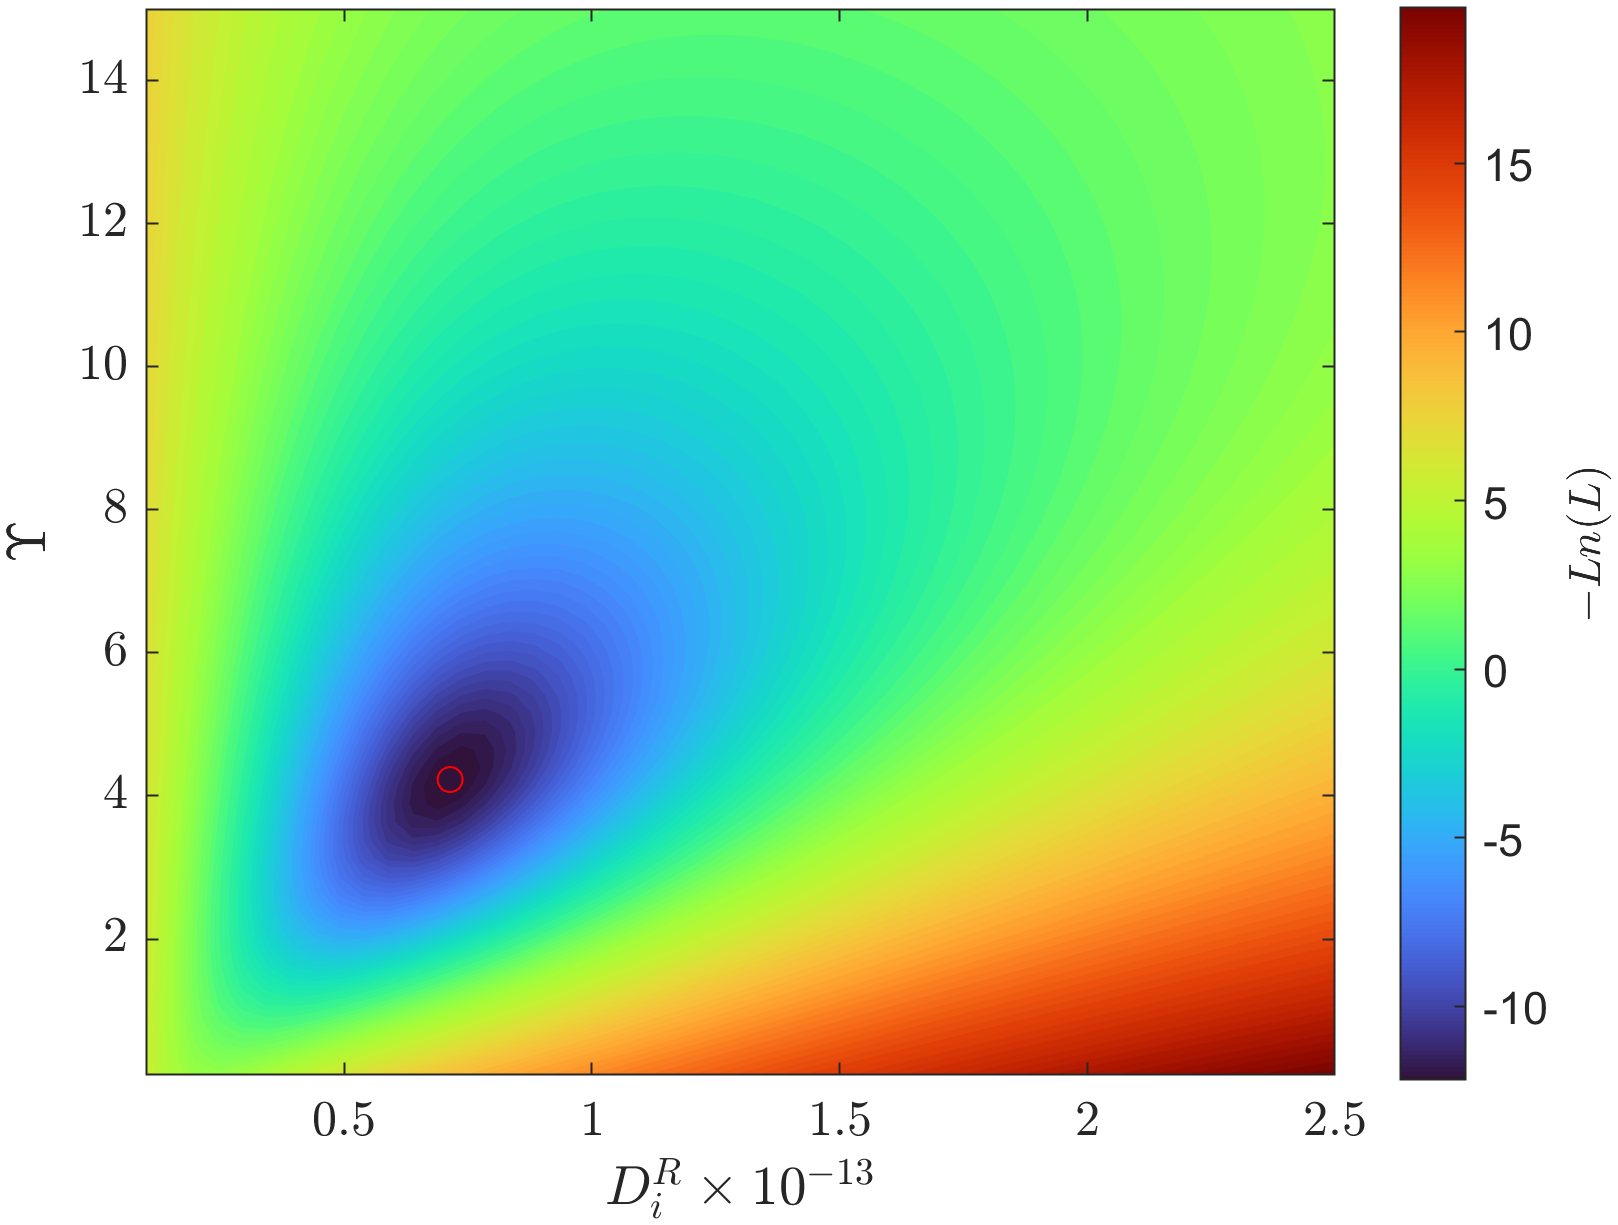
\includegraphics[trim = 0.0cm 0.0cm 0.0cm 0.0cm,clip, width=\columnwidth]{/Results_estimation/Parameter_space_Di_Gamma_dataset_1_org.png}
		\caption{Parameter space for the modified extraction model and experiment 1}
		\label{fig: Fit_1_Di_Gamma}
	\end{figure}
	
	The parameter space of the modified model is characterized by the unique minimum value, which corresponds to the solution of the parameter estimation problem for experiment 1. The red circle shows the minimum value of the cost function found by the optimizer. The remaining experiments are fitted to the modified extraction model, and results are presented in Figure \ref{fig: Fit_Di_Gamma}. The obtained results show good agreement with experimental data. 

	\begin{figure}[!h]
		\centering
		\begin{subfigure}[b]{\columnwidth}
			\centering
			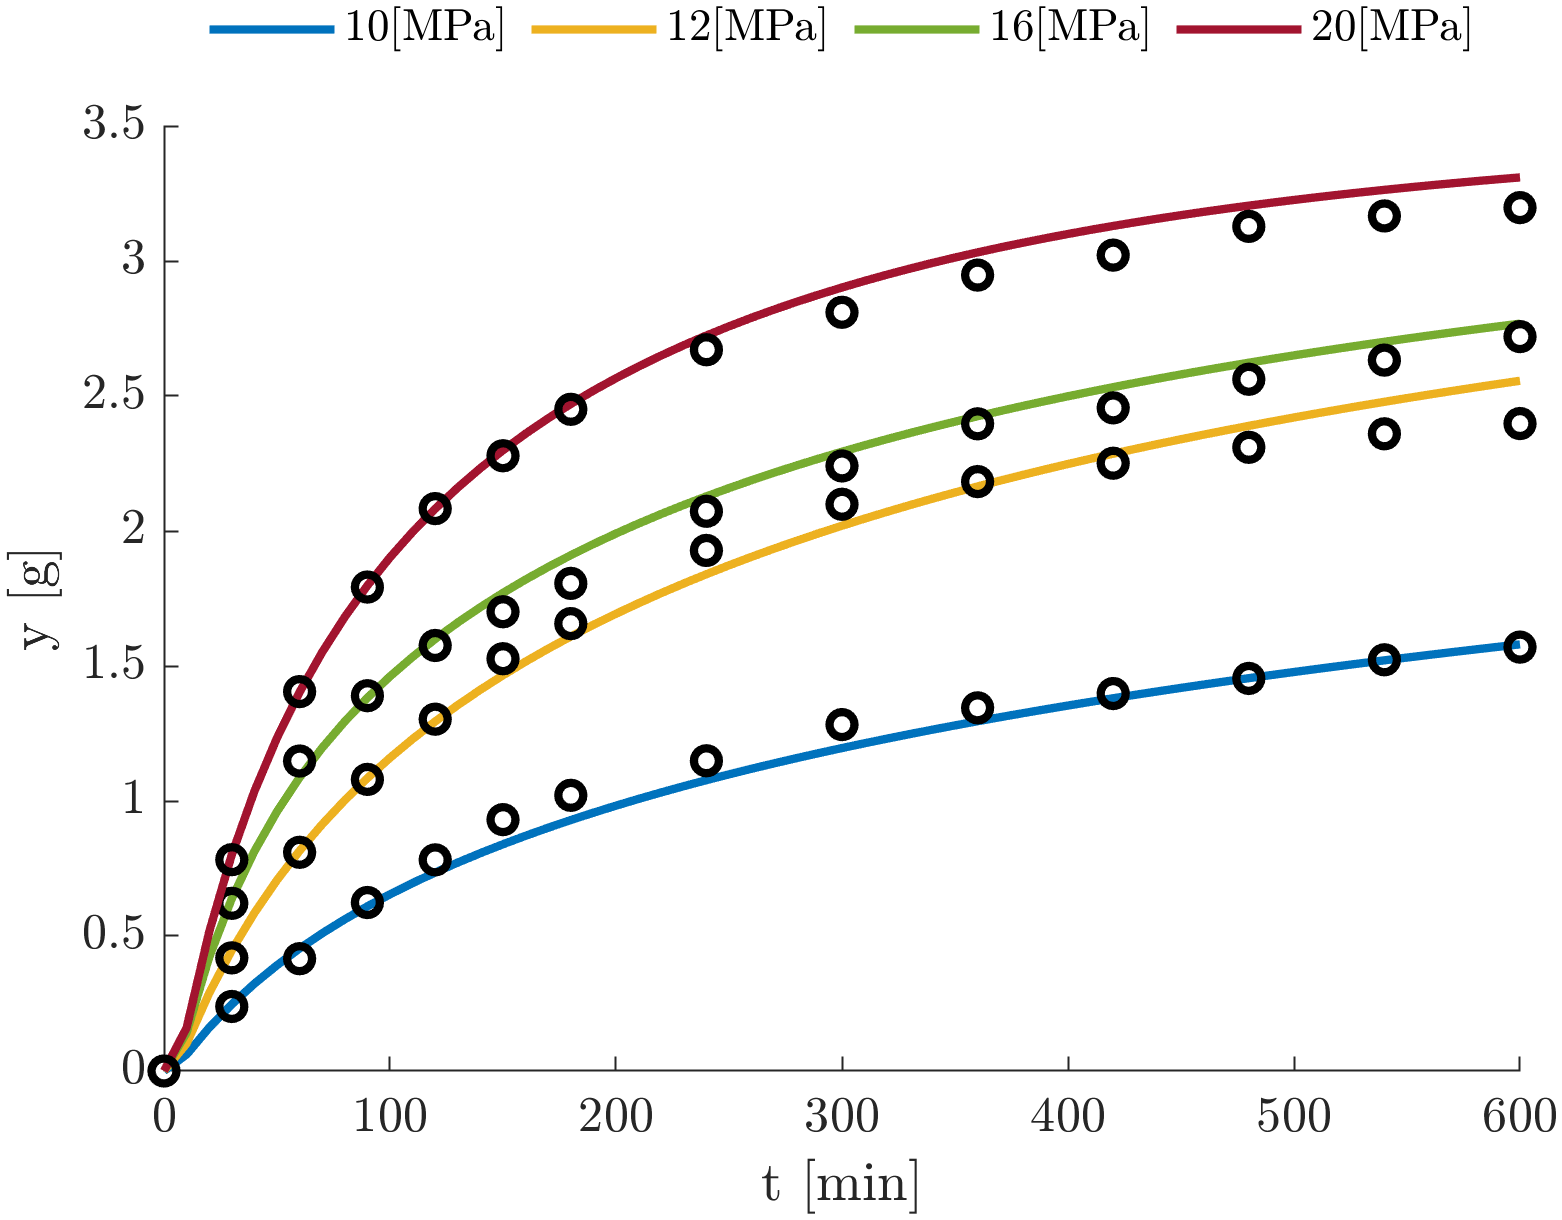
\includegraphics[trim = 0.0cm 0.0cm 0.0cm 0.0cm,clip, width=\columnwidth]{/Results_estimation/Fit_Di_Gamma_1_4.png}
			\caption{Results of parameter estimation for experiments at $6.67\times 10^{-5}$ [kg/s] and temperature of 40 $[^\circ C]$}
			\label{fig: Fit_1_4_Di_Gamma}
		\end{subfigure}
		\hfill
		\begin{subfigure}[b]{\columnwidth}
			\centering
			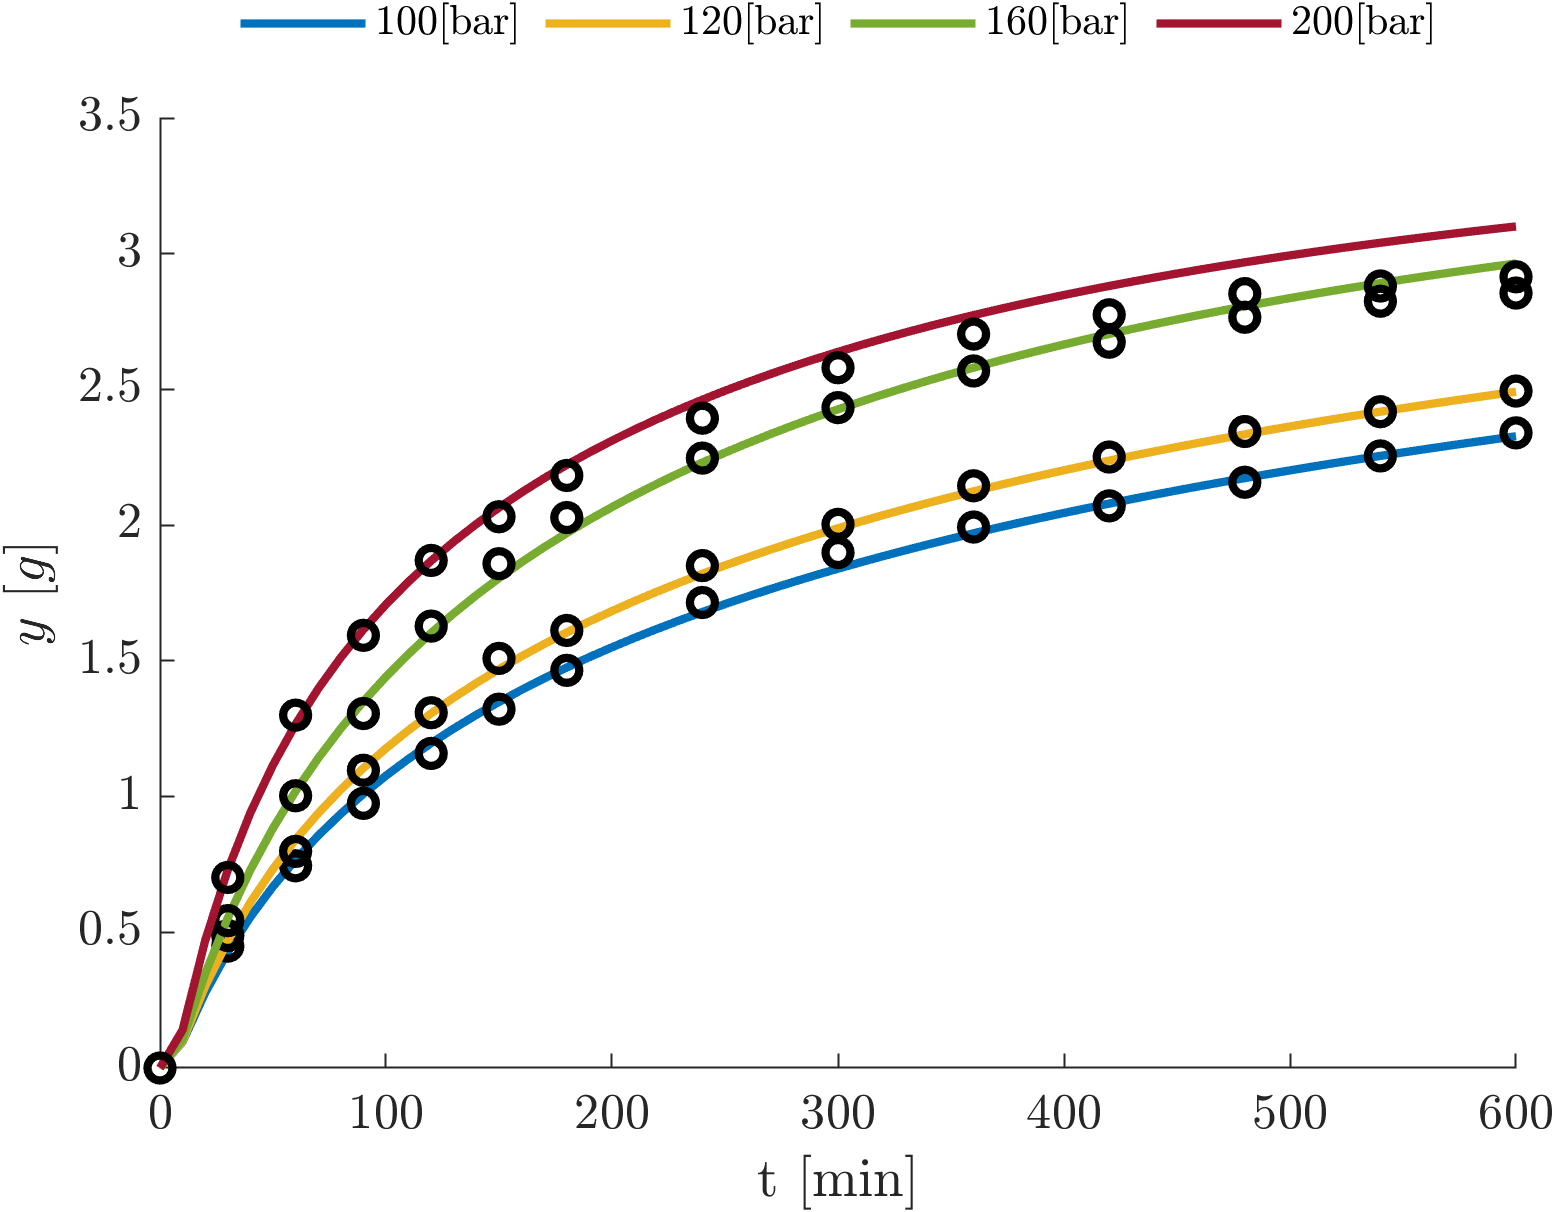
\includegraphics[trim = 0.0cm 0.0cm 0.0cm 0.0cm,clip, width=\columnwidth]{/Results_estimation/Fit_Di_Gamma_5_8.png}
			\caption{Results of parameter estimation for experiments at $6.67\times 10^{-5}$ [kg/s] and temperature of 30 $[^\circ C]$}
			\label{fig: Fit_5_8_Di_Gamma}
		\end{subfigure}
		\hfil
		\begin{subfigure}[b]{\columnwidth}
			\centering
			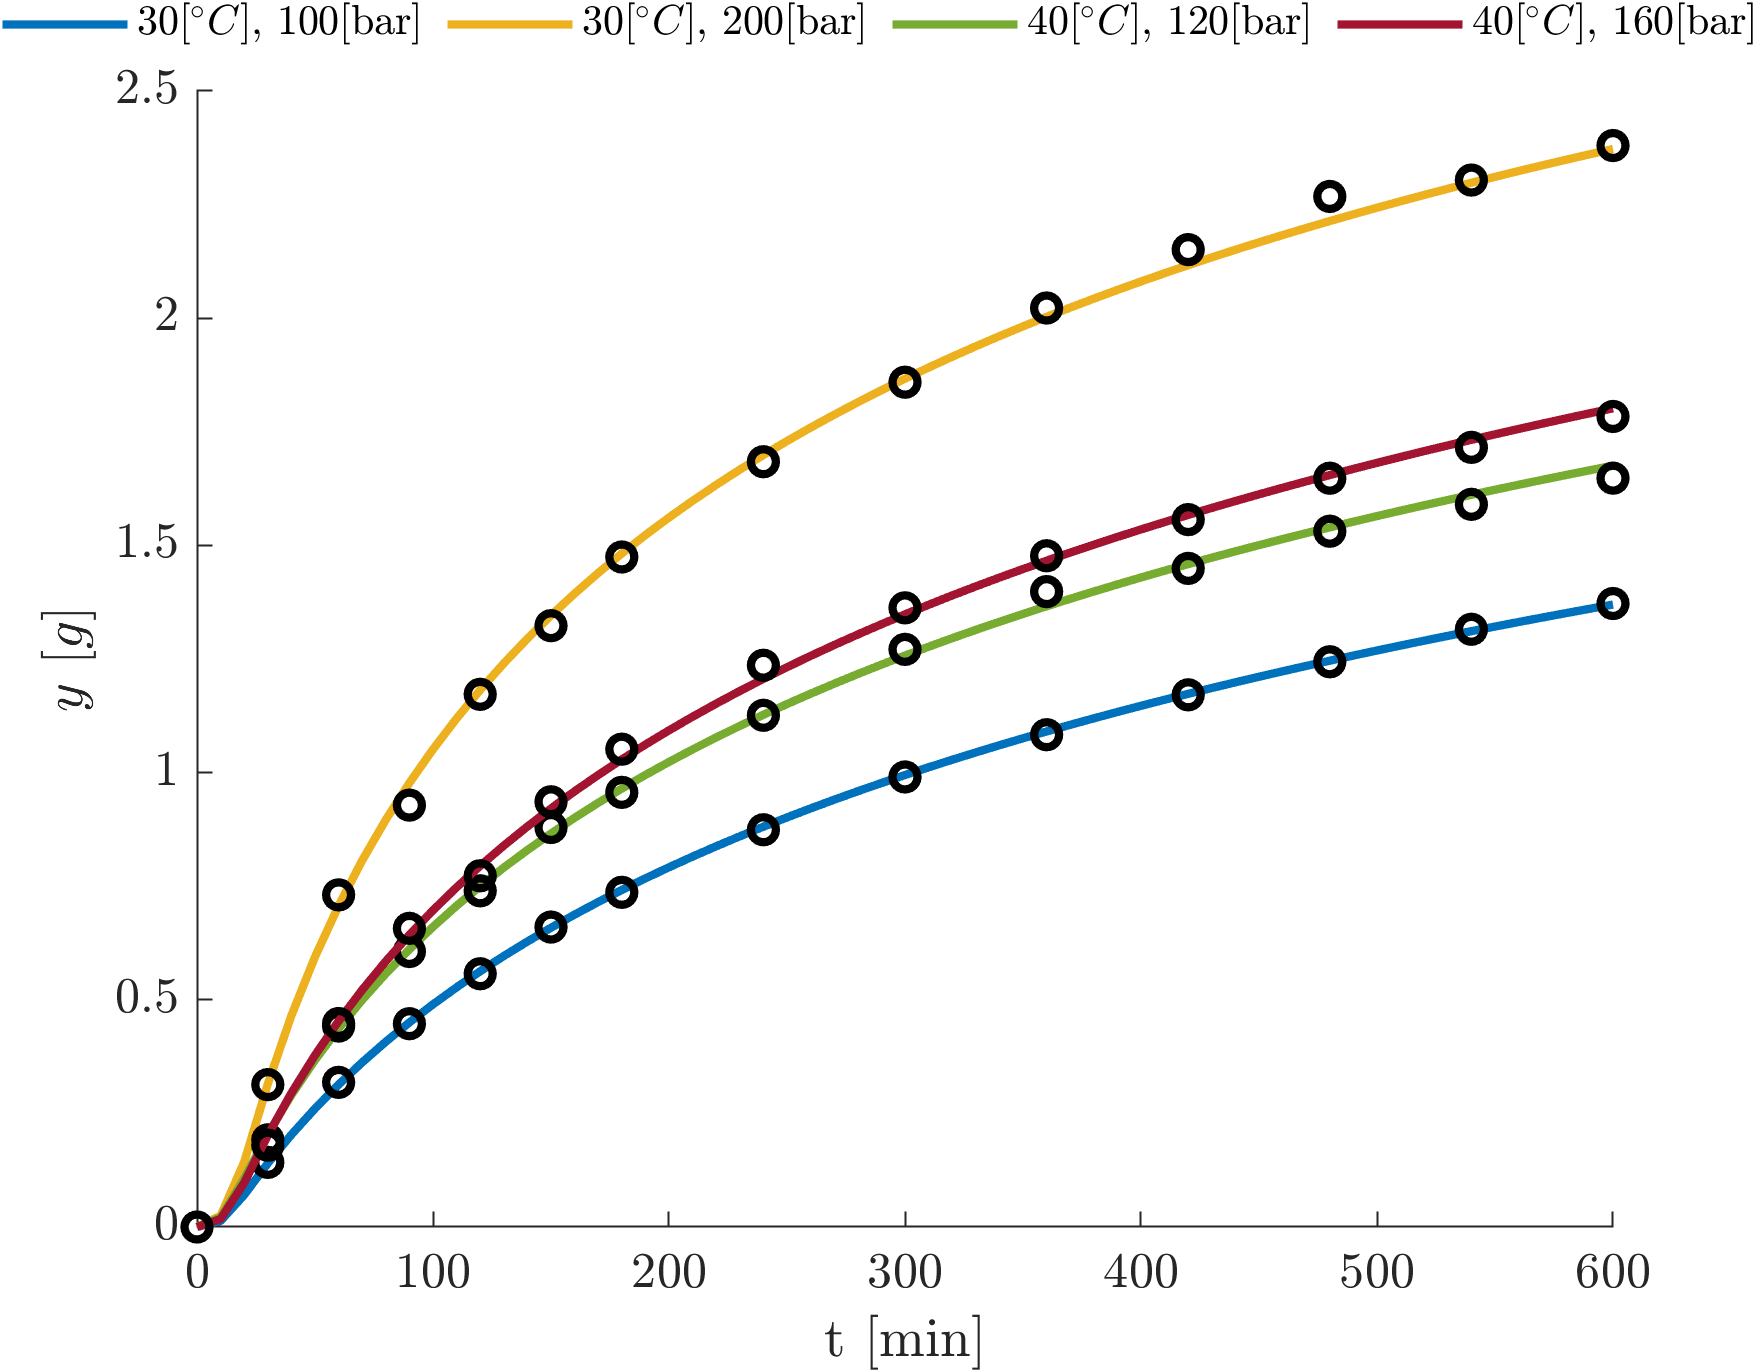
\includegraphics[trim = 0.0cm 0.0cm 0.0cm 0.0cm,clip, width=\columnwidth]{/Results_estimation/Fit_Di_Gamma_9_12.png}
			\caption{Results of parameter estimation for experiments at $3.33\times 10^{-5}$ [kg/s]}
			\label{fig: Fit_9_12_Di_Gamma}
		\end{subfigure}
		\caption{Parameter estimation results}
		\label{fig: Fit_Di_Gamma}
	\end{figure}
	
	The estimated parameters describe the decaying rate of internal diffusion coefficient $D_i$ according to Equation \ref{EQ: C_sat_function}. The internal diffusion coefficient is assumed to decrease as it is more difficult for a solute particle to diffuse from a particle core than the particle of a solute located next to the surface. The obtained decaying patterns are present in Figure \ref{fig: Gamma_function}. It can be noticed from the plot that a higher internal diffusion coefficient characterises the high-pressure fluid. This is in agreement with the work of \citet{Giddings1968}, \citet{Gurdial1989} and \citet{Machida2011} who analysed the solvation power of a solvent and correlated it with physical properties of $CO_2$. The Hildebrand solubility parameter was used to measure the cohesive energy density of a substance. \citet{Giddings1968} proposed a correlation for a solubility parameter $\delta_H[\text{MPa}^{1/2}] = 1.25 P_c^{1/2}\rho_r$, where $P_c$ and $\rho_r$ are critical pressure and reduced density respectively. \citet{Marcus2006} derived a similar correlation from the Van der Waals equation of state: $\delta_H[\text{MPa}^{1/2}] = 2.79 P_c^{1/4}T_r^{1/4}\rho_r$. Figure \ref{fig: Gamma_function} shows that fluid characterised by a higher solubility factor has larger values of internal diffusion coefficient. The relation between $\delta_H$ and $D_i$ should only be treated as an indicator because the system is non-ideal, and external factors such as fluid velocity are not considered.
	
	\begin{figure}[!h]
		\centering
		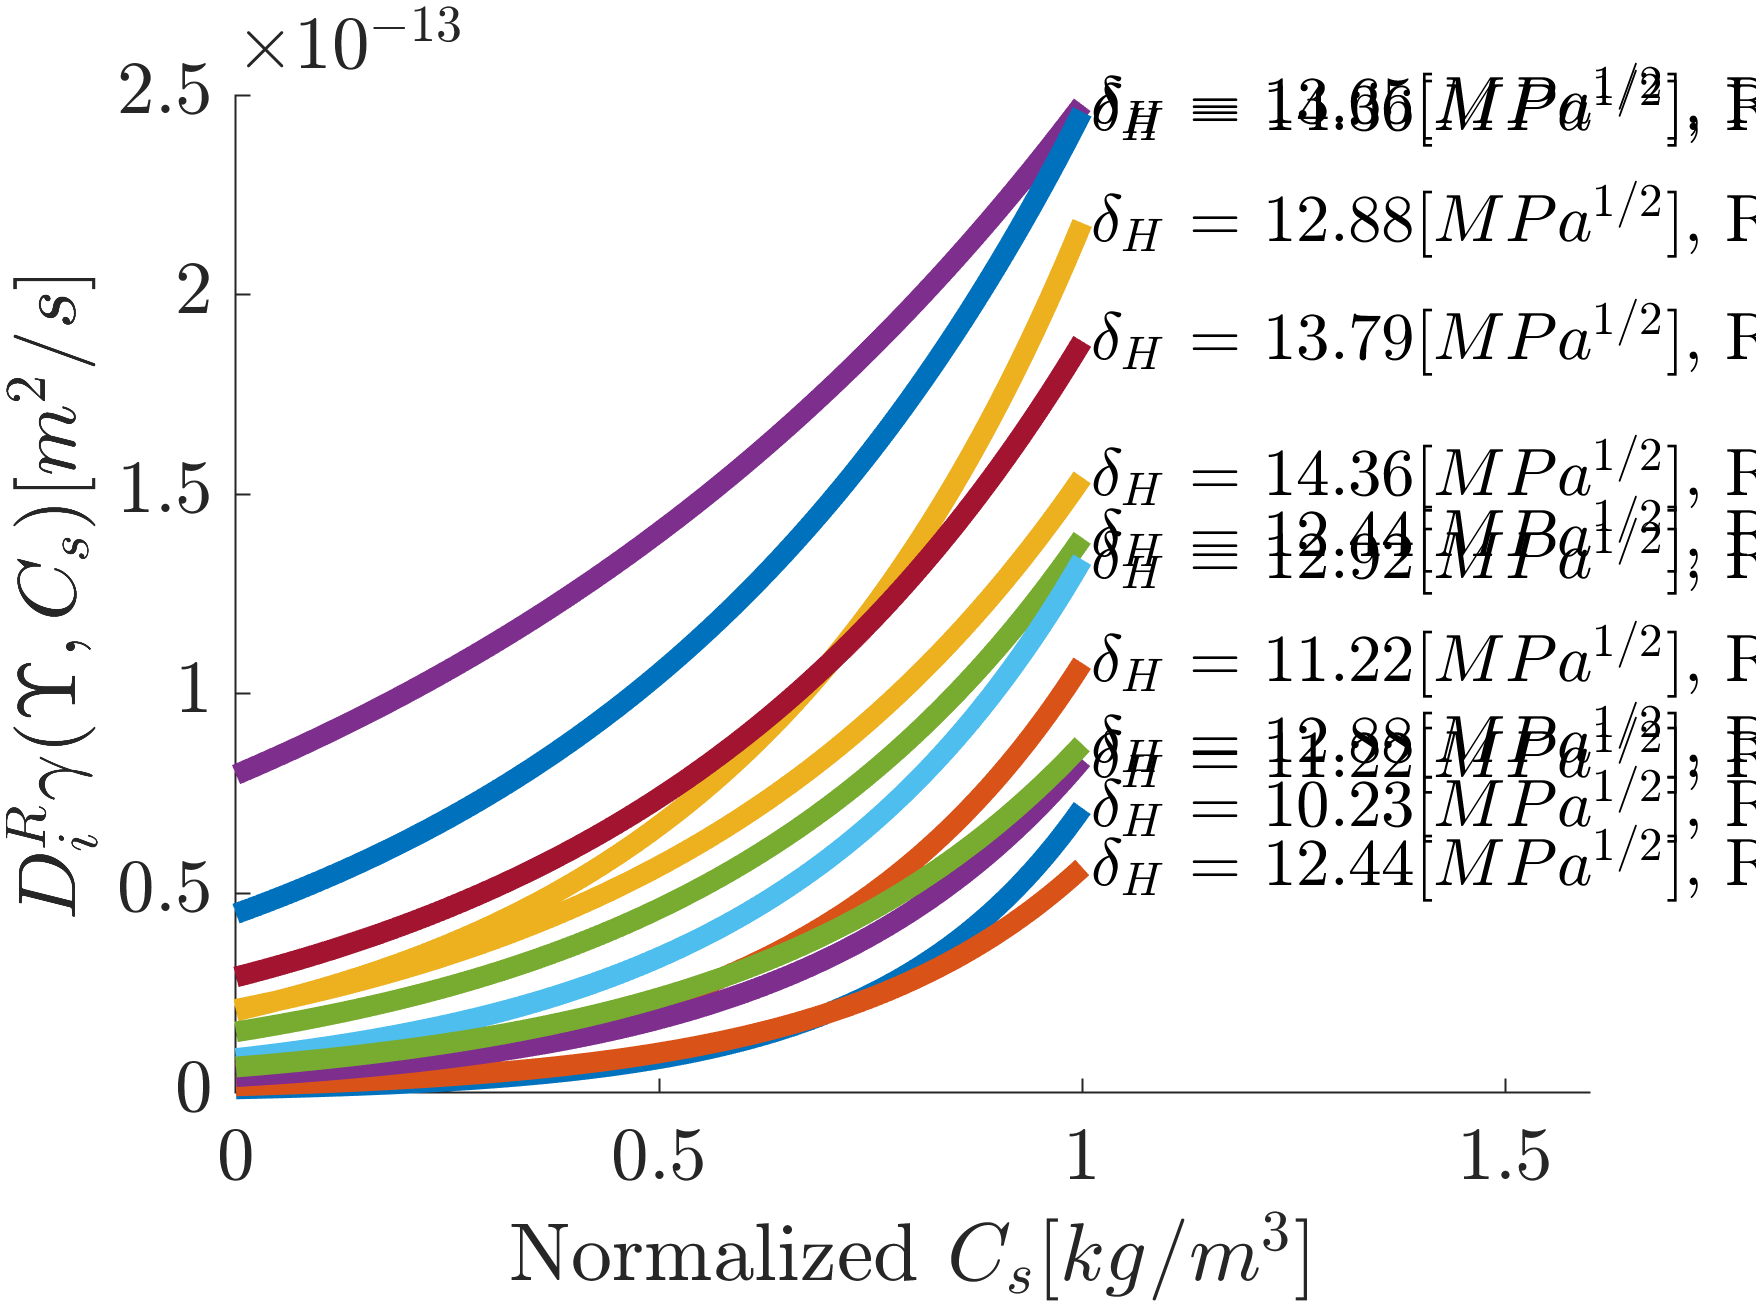
\includegraphics[trim = 0.0cm 0.0cm 0.0cm 0.0cm,clip, width=\columnwidth]{/Results_estimation/Gamma_function.png}
		\caption{The decaying internal diffusion coefficient}
		\label{fig: Gamma_function}
	\end{figure}
		
	The parameter estimation results are combined to analyse the relationship between the obtained parameters and the operating conditions. This work does not apply the traditional approach for finding correlations by combining Reynolds, Schmidt and Sherwood numbers because the axial diffusion was considered negligible. Instead, the Reynolds number $\left(Re = \frac{(2r) \cdot \rho_f \cdot u}{\mu}\right)$ is used solely as an independent variable as shown in Figure \ref{fig: Correlations}. Using the Reynolds number has the advantage of considering the influence of all the control variables (temperature, pressure and flow rate), which means it can be uniquely defined by selecting operating conditions.	
	Two data clusters can be distinguished in Figures \ref{fig: Correlations_Di_Re} and \ref{fig: Correlations_Gamma_Re}, where each cluster corresponds to a different mass flow rate. Even though a linear trend characterises both correlations, correlations related to $D_i^R$ decrease with Re while the correlations related to $\Upsilon$ increase with Re. Higher fluid density and corresponding mass transfer resistance can explain the decrease of the $D_i^R$ along each line. On the other hand, the increase in $\Upsilon$ correlations can be justified by higher solubility. The Hildebrand solubility factor is mainly a function of fluid density, which is also present in the the Reynolds number hence $\Upsilon$ can be correlated with Re.
	
	\begin{figure}[!h]
		\centering
		\begin{subfigure}[b]{\columnwidth}
			\centering
			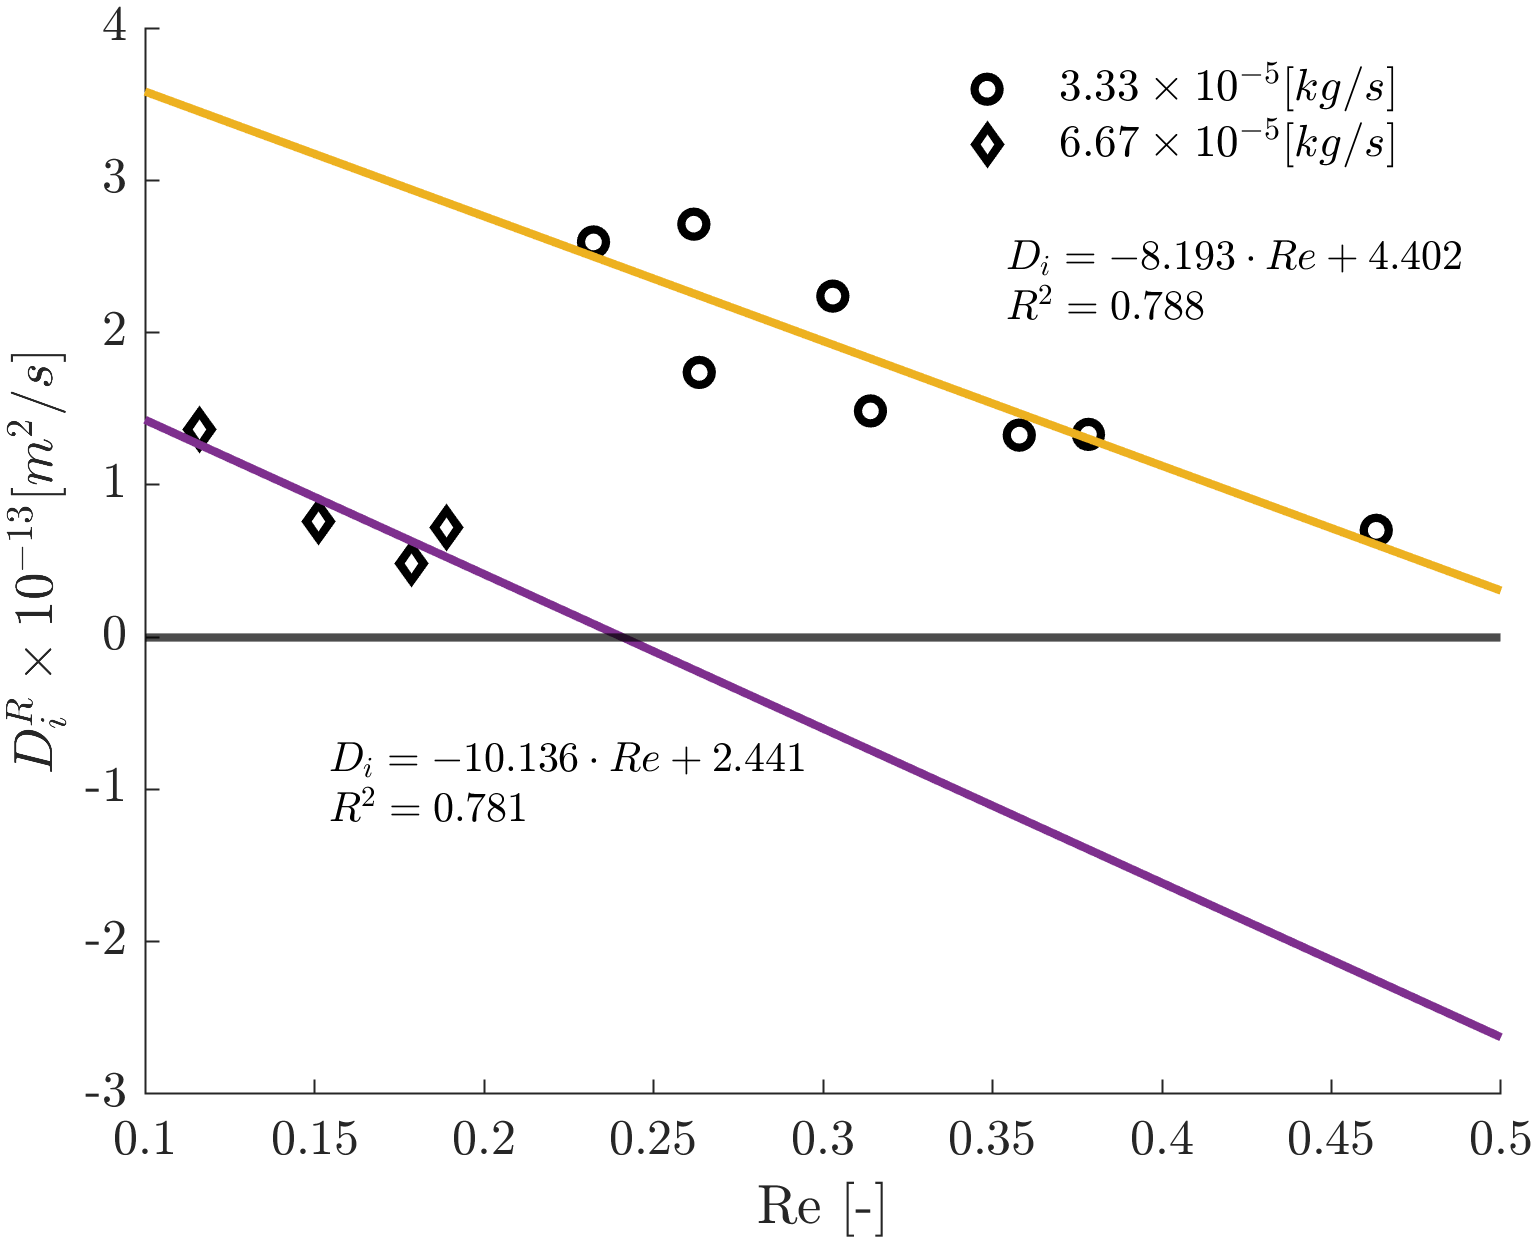
\includegraphics[trim = 0.0cm 0.0cm 0.0cm 0.0cm,clip, width=\columnwidth]{/Results_estimation/Correlation_Di_Re.png}
			\caption{Linear regression $D_i^R = f(Re)$}
			\label{fig: Correlations_Di_Re}
		\end{subfigure}
		\hfill
		\begin{subfigure}[b]{\columnwidth}
			\centering
			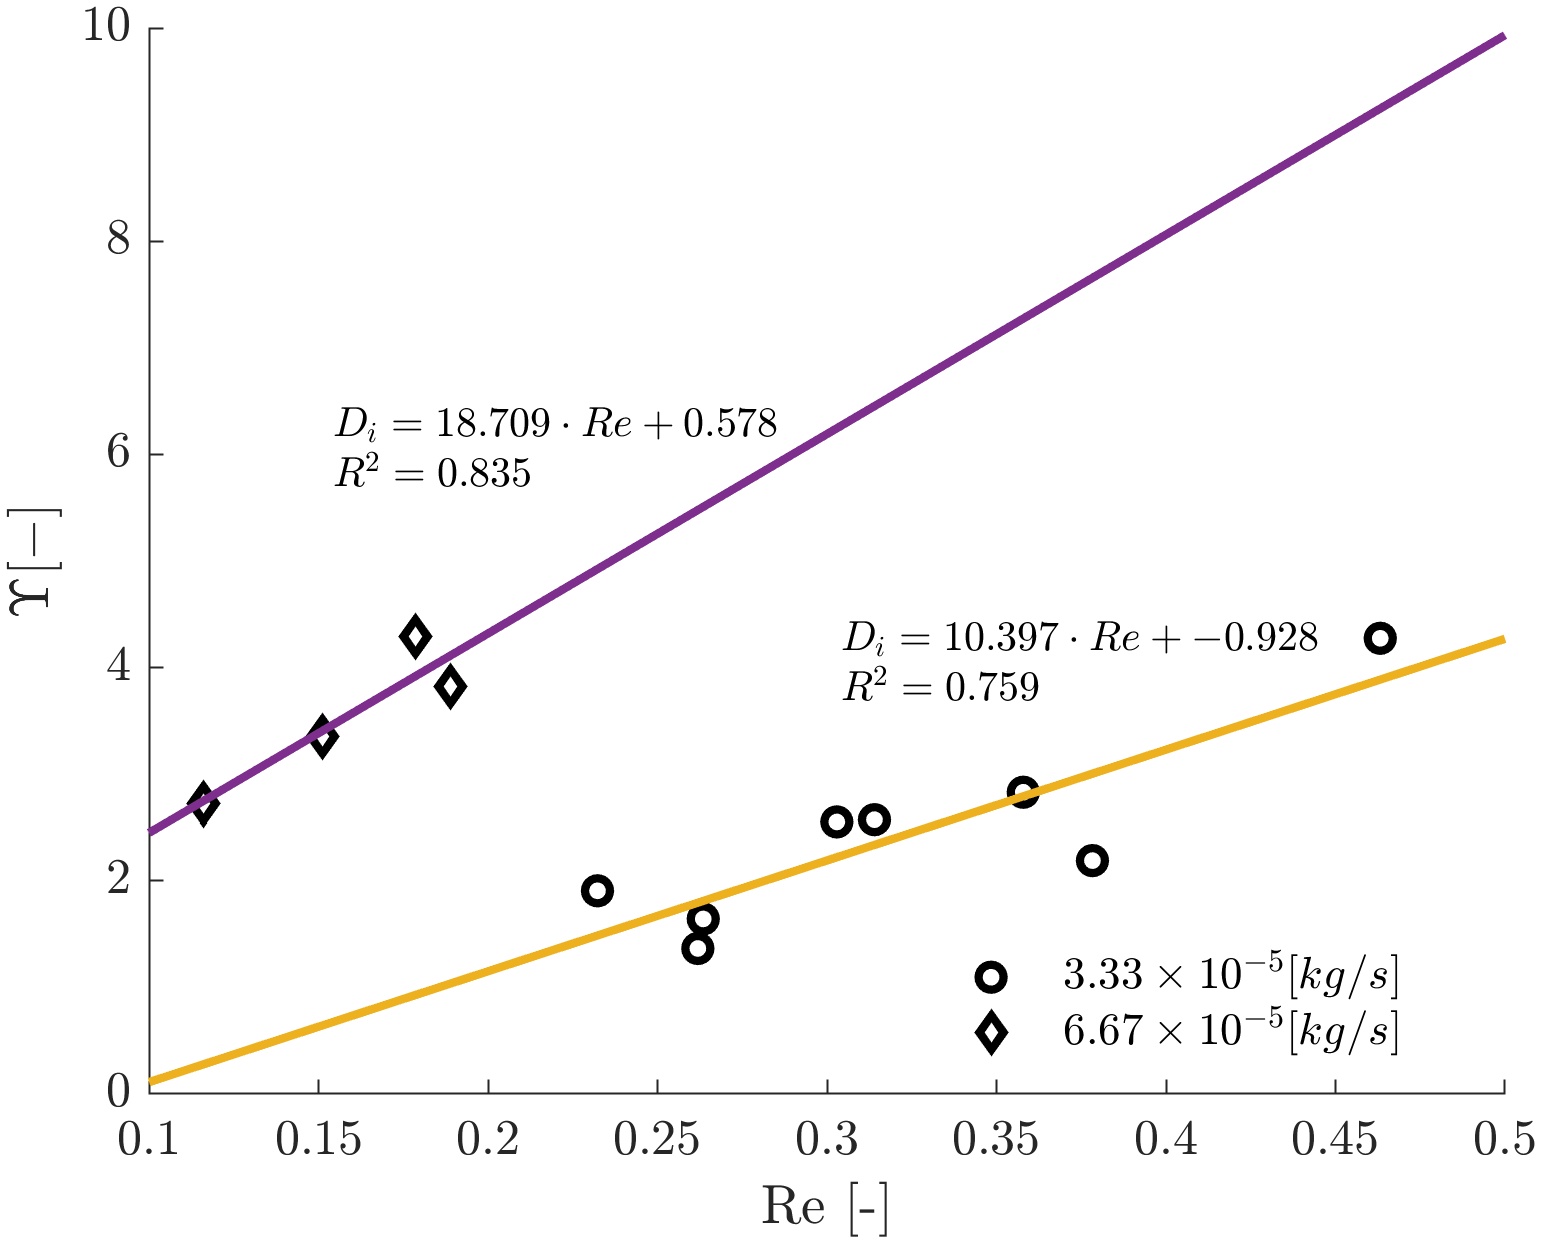
\includegraphics[trim = 0.0cm 0.0cm 0.0cm 0.0cm,clip, width=\columnwidth]{/Results_estimation/Correlation_Gamma_Re.png}
			\caption{Linear regression $\Upsilon = f(Re)$}
			\label{fig: Correlations_Gamma_Re}
		\end{subfigure}
		\caption{Parameter estimation results}
		\label{fig: Correlations}
	\end{figure}
	
\end{document}